

%% AAPT Physics Bowl Exams Questions
%%----------------------------------------


%% This section has XX problems


%% PhysicsBowl 2015
%%----------------------------------------
\element{aapt}{ %% Bowl-B1
\begin{question}{bowl-2015-q04}
    A standing wave on a string is produced.
    Which one of the following choices best describes the location
        on the string at which maximum constructive interference occurs?
    \begin{multicols}{2}
    \begin{choices}
        \wrongchoice{node}
      \correctchoice{antinode}
        \wrongchoice{harmonic}
        \wrongchoice{overtone}
        \wrongchoice{amplitude}
    \end{choices}
    \end{multicols}
\end{question}
}


%% PhysicsBowl 2014
%%----------------------------------------
\element{aapt1}{ %% Bowl-B1
\begin{question}{bowl-2014-q01}
    An FM radio station sends a signal with a frequency
        of \SI{99.99e6}{\hertz}.
    Which one of the following choices best represents
        this frequency expressed using metric prefixes?
    \begin{multicols}{2}
    \begin{choices}
        \wrongchoice{\SI{99.99}{\kilo\hertz}.}
      \correctchoice{\SI{99.99}{\mega\hertz}.}
        \wrongchoice{\SI{99.99}{\giga\hertz}.}
        \wrongchoice{\SI{99.99}{\tera\hertz}.}
        \wrongchoice{\SI{99.99}{\nano\hertz}.}
    \end{choices}
    \end{multicols}
\end{question}
}


%% PhysicsBowl 2012
%%----------------------------------------
\element{aapt}{ %% Bowl-B1
\begin{question}{bowl-2012-q04}
    The wave speed is \SI{20.0}{\meter\per\second}
        for waves traveling on a string tied at both ends.
    If sinusoidal waves with a frequency of \SI{2.00}{\hertz}
        are traveling on this string, which one of the
        following choices best represents the period
        of these waves?
    \begin{multicols}{3}
    \begin{choices}
        \wrongchoice{\SI{40.0}{\second}}
        \wrongchoice{\SI{10.0}{\second}}
        \wrongchoice{\SI{3.16}{\second}}
      \correctchoice{\SI{0.50}{\second}}
        \wrongchoice{\SI{0.10}{\second}}
    \end{choices}
    \end{multicols}
\end{question}
}


%% PhysicsBowl 2011
%%----------------------------------------
\element{aapt}{ %% Bowl-B1
\begin{question}{bowl-2011-q17}
    A new radio station broadcasts its signal with a wavelength of \SI{3.40}{\meter}.
    At what frequency is this station broadcasting?
    \begin{multicols}{2}
    \begin{choices}
        \wrongchoice{\SI{1.76e8}{\hertz}}
      \correctchoice{\SI{8.82e7}{\hertz}}
        \wrongchoice{\SI{100}{\hertz}}
        \wrongchoice{\SI{0.294}{\hertz}}
        \wrongchoice{\SI{1.13e-8}{\hertz}}
    \end{choices}
    \end{multicols}
\end{question}
}

\element{aapt}{ %% Bowl-B1
\begin{question}{bowl-2011-q23}
    A string, clamped at both ends, has its tension fixed.
    A wave generator vibrates the string with a frequency $f$ producing waves of wavelength $\lambda$ which have speed $v$.
    The frequency of the wave generator is now doubled to $2f$.
    Which one of the following choices best describes the new value of the wavelength of waves produced and the speed of the waves on the string?
    \begin{center}
    \begin{tabu}{cX[c]X[c]}
        \toprule
        \makebox[1.5em][c]{\textnumero}
            & Wavelength & Wave speed \\
        \bottomrule
    \end{tabu}
    \end{center}
    \begin{choices}
      \correctchoice{\begin{tabu}{X[c]X[c]} $\dfrac{\lambda}{2}$  & $v$ \\ \end{tabu}}
        \wrongchoice{\begin{tabu}{X[c]X[c]} $\dfrac{\lambda}{2}$ & $2v$ \\ \end{tabu}}
        \wrongchoice{\begin{tabu}{X[c]X[c]} $\lambda$  & $2v$ \\ \end{tabu}}
        \wrongchoice{\begin{tabu}{X[c]X[c]} $\lambda$ & $v$ \\ \end{tabu}}
        \wrongchoice{\begin{tabu}{X[c]X[c]} $2\lambda$ & $4v$ \\ \end{tabu}}
    \end{choices}
\end{question}
}

\element{aapt}{ %% Bowl-B1
\begin{question}{bowl-2011-q24}
    Two waves pulses travel to the right toward a rigid boundary as shown.
    \begin{center}
    \begin{tikzpicture}
        \draw[thin,dashed,white!90!black,step=0.5] (0,-1) grid (6,2);
        %% Two waves
        \draw[ultra thick] (0,0) -- (1,0) -- (1,1) -- (3,1) -- (3,0) -- (4,0) -- (5,1) -- (5,0) -- (6,0);
        %% thick wall
        \draw (6,-1) -- (6,2);
        \node[anchor=west,pattern=north east lines,minimum height=3cm] at (6,0.5) {};
        %% vectors
        \draw[ultra thick,-latex] (1.5,1.5) -- ++(0:1);
        \draw[ultra thick,-latex] (4,1.5) -- ++(0:1);
    \end{tikzpicture}
    \end{center}
    After reflection of the triangular pulse,
        the pulses will interfere.
    Which one of the following pictures best represents the superposition of the pulses when the centers of the individual pulses coincide?
    \begin{multicols}{2}
    \begin{choices}
        \AMCboxDimensions{down=-0.4cm}
        \correctchoice{
            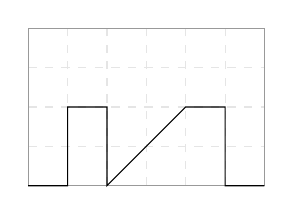
\begin{tikzpicture}
                \draw[thin,dashed,white!90!black,step=0.5] (0,0) grid (3,2);
                \draw[thin,white!60!black] (0,0) rectangle (3,2);
                \draw (0,0) -- (0.5,0) -- (0.5,1) -- (1,1) -- (1,0) -- (2,1) -- (2.5,1) -- (2.5,0) -- (3,0);
            \end{tikzpicture}
        }
        \wrongchoice{
            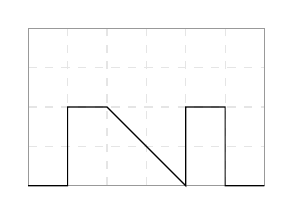
\begin{tikzpicture}
                \draw[thin,dashed,white!90!black,step=0.5] (0,0) grid (3,2);
                \draw[thin,white!60!black] (0,0) rectangle (3,2);
                \draw (0,0) -- (0.5,0) -- (0.5,1) -- (1,1) -- (2,0) -- (2,1) -- (2.5,1) -- (2.5,0) -- (3,0);
            \end{tikzpicture}
        }
        \wrongchoice{
            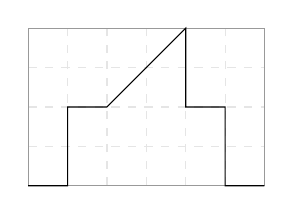
\begin{tikzpicture}
                \draw[thin,dashed,white!90!black,step=0.5] (0,0) grid (3,2);
                \draw[thin,white!60!black] (0,0) rectangle (3,2);
                \draw (0,0) -- (0.5,0) -- (0.5,1) -- (1,1) -- (2,2) -- (2,1) -- (2.5,1) -- (2.5,0) -- (3,0);
            \end{tikzpicture}
        }
        \wrongchoice{
            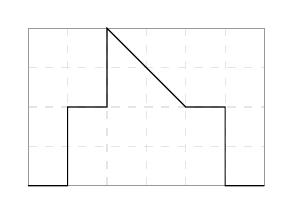
\begin{tikzpicture}
                \draw[thin,dashed,white!90!black,step=0.5] (0,0) grid (3,2);
                \draw[thin,white!60!black] (0,0) rectangle (3,2);
                \draw (0,0) -- (0.5,0) -- (0.5,1) -- (1,1) -- (1,2) -- (2,1) -- (2.5,1) -- (2.5,0) -- (3,0);
            \end{tikzpicture}
        }
        \wrongchoice{
            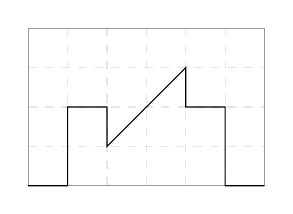
\begin{tikzpicture}
                \draw[thin,dashed,white!90!black,step=0.5] (0,0) grid (3,2);
                \draw[thin,white!60!black] (0,0) rectangle (3,2);
                \draw (0,0) -- (0.5,0) -- (0.5,1) -- (1,1) -- (1,0.5) -- (2,1.5) -- (2,1) -- (2.5,1) -- (2.5,0) -- (3,0);
            \end{tikzpicture}
        }
    \end{choices}
    \end{multicols}
\end{question}
}


%% PhysicsBowl 2009
%%----------------------------------------
\element{aapt}{ %% Bowl-B1
\begin{question}{bowl-2009-q06}
    For a standing wave mode on a string fixed at both ends,
        adjacent antinodes are separated by a distance of \SI{20}{\centi\meter}.
    Waves travel on this string at a speed of \SI{1200}{\centi\meter\per\second}.
    At what frequency is the string vibrated to produce this standing wave?
    \begin{multicols}{3}
    \begin{choices}
        \wrongchoice{\SI{120}{\joule}}
        \wrongchoice{\SI{60}{\joule}}
        \wrongchoice{\SI{40}{\joule}}
      \correctchoice{\SI{30}{\joule}}
        \wrongchoice{\SI{20}{\joule}}
    \end{choices}
    \end{multicols}
\end{question}
}


%% PhysicsBowl 2008
%%----------------------------------------
\element{aapt}{ %% Bowl-B1
\begin{question}{bowl-2008-q46}
    A traveling wave has the form
    \begin{equation*}
        y(x,t) = \num{3.0}\sin\left(\num{2.5}x - \num{5.0}t \right)
    \end{equation*}
    where all quantities given are in MKS units,
        $X$ is position, and $T$ represents time.
    What is the period of the wave?
    \begin{multicols}{3}
    \begin{choices}
        \wrongchoice{\SI{2.00}{\second}}
      \correctchoice{\SI{1.26}{\second}}
        \wrongchoice{\SI{1.00}{\second}}
        \wrongchoice{\SI{0.63}{\second}}
        \wrongchoice{\SI{0.20}{\second}}
    \end{choices}
    \end{multicols}
\end{question}
}


%% PhysicsBowl 2007
%%----------------------------------------
\element{aapt}{ %% Bowl-B1
\begin{question}{bowl-2007-q37}
    A place of zero displacement on a standing wave is called:
    \begin{multicols}{2}
    \begin{choices}
        \wrongchoice{an antinode}
      \correctchoice{an node}
        \wrongchoice{the amplitude}
        \wrongchoice{the wavenumber}
        \wrongchoice{the harmonic}
    \end{choices}
    \end{multicols}
\end{question}
}

\element{aapt}{ %% Bowl-B1
\begin{question}{bowl-2007-q44}
    A person vibrates the end of a string sending transverse waves down the string.
    If the person then doubles the rate at which he vibrates the string,
        the speed of the waves
    \begin{choices}
        \wrongchoice{doubles and the wavelength is unchanged.}
        \wrongchoice{doubles and the wavelength doubled.}
        \wrongchoice{doubles while the wavelength is halved.}
        \wrongchoice{is unchanged while the wavelength is doubled.}
      \correctchoice{is unchanged while the wavelength is halved.}
    \end{choices}
\end{question}
}


%% PhysicsBowl 2005
%%----------------------------------------
\element{aapt}{ %% Bowl-B1
\begin{question}{bowl-2005-q01}
    Which quantity is \emph{not} a scalar?
    \begin{multicols}{2}
    \begin{choices}
      \correctchoice{velocity}
        \wrongchoice{speed}
        \wrongchoice{wavelength}
        \wrongchoice{specific heat}
        \wrongchoice{temperature}
    \end{choices}
    \end{multicols}
\end{question}
}


%% PhysicsBowl 2000
%%----------------------------------------
\element{aapt}{ %% Bowl-B1
\begin{question}{bowl-2000-q07}
    The length of the most effective transmitting antenna is equal to one-fourth the wavelength of the broadcast wave.
    If a radio station has an antenna \SI{4.5}{\meter} long then what is the broadcast frequency of the radio station?
    \begin{multicols}{2}
    \begin{choices}
        \wrongchoice{\SI{1.5e-8}{\hertz}}
        \wrongchoice{\SI{6.0e-8}{\hertz}}
        \wrongchoice{\SI{1.7e7}{\hertz}}
        \wrongchoice{\SI{6.7e7}{\hertz}}
      \correctchoice{\SI{3.0e8}{\hertz}}
    \end{choices}
    \end{multicols}
\end{question}
}


%% PhysicsBowl 1999
%%----------------------------------------
\element{aapt}{ %% Bowl-B1
\begin{question}{bowl-1999-q25}
    Pioneering radio station KFKA started broadcasting
        \SI{78}{\year} ago at 1310 (\SI{1.31}{\mega\hertz}) on the AM dial.
    What is the approximate length of its radio waves?
    \begin{multicols}{2}
    \begin{choices}
        \wrongchoice{\SI{23}{\meter}}
      \correctchoice{\SI{230}{\meter}}
        \wrongchoice{\SI{2 300}{\meter}}
        \wrongchoice{\SI{23 000}{\meter}}
        \wrongchoice{\SI{3e8}{\meter}}
    \end{choices}
    \end{multicols}
\end{question}
}

\element{aapt}{ %% Bowl-B1
\begin{question}{bowl-1999-q27}
    Assume that waves are propagating in a uniform medium.
    If the frequency of the wave source doubles then:
    \begin{choices}
        \wrongchoice{The speed of the waves doubles}
        \wrongchoice{The wavelength of the waves doubles}
        \wrongchoice{The speed of the waves halves}
      \correctchoice{The wavelength of the waves halves}
        \wrongchoice{None of the provided}
    \end{choices}
\end{question}
}


%% PhysicsBowl 1998
%%----------------------------------------
\element{aapt}{ %% Bowl-B1
\begin{question}{bowl-1998-q02}
    An observer hears a sound with frequency \SI{400}{\hertz}.
    Its wavelength is approximately:
    \begin{multicols}{3}
    \begin{choices}
      \correctchoice{\SI{0.85}{\meter}}
        \wrongchoice{\SI{1.2}{\meter}}
        \wrongchoice{\SI{2.75}{\meter}}
        \wrongchoice{\SI{13.6}{\meter}}
        \wrongchoice{\SI{44}{\meter}}
    \end{choices}
    \end{multicols}
\end{question}
}


%% PhysicsBowl 1997
%%----------------------------------------
\element{aapt}{ %% Bowl-B1
\begin{question}{bowl-1997-q04}
    Which station broadcasts with \SI{3.27}{\meter} radio waves?
    \begin{multicols}{2}
    \begin{choices}
      \correctchoice{\SI{91.7}{\mega\hertz}}
        \wrongchoice{\SI{92.5}{\mega\hertz}}
        \wrongchoice{\SI{98.5}{\mega\hertz}}
        \wrongchoice{\SI{102.5}{\mega\hertz}}
        \wrongchoice{\SI{106.3}{\mega\hertz}}
    \end{choices}
    \end{multicols}
\end{question}
}

\element{aapt}{ %% Bowl-B1
\begin{question}{bowl-1997-q19}
    The standing wave pattern diagrammed to the right is produced in a string fixed at both ends.
    %% NOTE: bowl-1994-q19
    \begin{center}
    \begin{tikzpicture}[x=0.07\linewidth]
        %% walls
        \draw (0,1) -- (0,-1);
        \draw (12.56,1) -- (12.56,-1);
        \node[pattern=north east lines,anchor=east,minimum height=2cm] at (0,0) {};
        \node[pattern=north east lines,anchor=west,minimum height=2cm] at (12.56,0) {};
        %% waves
        \draw[thick,domain=0:4*pi,smooth,line width=1pt] plot (\x, {0.8*sin(\x r)});
        \draw[dashed,domain=0:4*pi,smooth,line width=1pt] plot (\x, {-0.8*sin(\x r)});
        %% distance
        \draw[<->] (0,-1.33) --  (12.56,-1.33) node[pos=0.5,anchor=center,fill=white] {\SI{1.0}{\meter}};
    \end{tikzpicture}
    \end{center}
    The speed of waves in the string is \SI{2.0}{\meter\per\second}.
    What is the frequency of the standing wave pattern
    \begin{multicols}{3}
    \begin{choices}
        \wrongchoice{\SI{0.25}{\hertz}}
        \wrongchoice{\SI{1.0}{\hertz}}
        \wrongchoice{\SI{2.0}{\hertz}}
      \correctchoice{\SI{4.0}{\hertz}}
        \wrongchoice{\SI{8.0}{\hertz}}
    \end{choices}
    \end{multicols}
\end{question}
}

\element{aapt}{ %% Bowl-B1
\begin{question}{bowl-1997-q23}
    String $L$ and string $H$ have the same tension and length.
    String $L$ has mass $m$ and string $H$ has mass $4m$.
    If the speed waves in string $L$ is $v$,
        the speed of waves in string $H$ is:
    \begin{multicols}{3}
    \begin{choices}
      \correctchoice{$\dfrac{v}{2}$}
        \wrongchoice{$v$}
        \wrongchoice{$\sqrt{2}\,v$}
        \wrongchoice{$\num{2}\,v$}
        \wrongchoice{$\num{4}\,v$}
    \end{choices}
    \end{multicols}
\end{question}
}


%% PhysicsBowl 1996
%%----------------------------------------
\element{aapt}{ %% Bowl-B1
\begin{question}{bowl-1996-q10}
    Two wave pulses approach each other as seen in the figure below.
    The wave pulses overlap at point $P$.
    \begin{center}
    \begin{tikzpicture}[scale=0.9]
        %% left wave
        \draw (0,0) -- (-1,0) -- (-1,0.5) -- (-3,0.5) -- (-3,0) -- (-4,0);
        \draw[thick,->] (-1.9,1) -- ++(0:1);
        %% right wave
        \draw (0,0) -- (1,0) -- (2,-1) -- (3,0) -- (4,0);
        \draw[thick,->] (1.9,-1) -- ++(180:1);
        %% right wave
        \fill (0,0) circle (2pt) node[anchor=north] {$P$};
    \end{tikzpicture}
    \end{center}
    Which diagram best represents the appearance of the wave pulses as they leave point $P$?
    \begin{choices}
        \AMCboxDimensions{down=-0.8cm}
        \wrongchoice{
            \begin{tikzpicture}[scale=0.9]
                \draw[dashed,white!90!black] (-4.1,-1.2) rectangle (4.1,1.2);
                %% left wave
                \draw (0,0) -- (-1,0) -- (-1,0.5) -- (-3,0.5) -- (-3,0) -- (-4,0);
                \draw[thick,->] (-2.1,1) -- ++(180:1);
                %% right wave
                \draw (0,0) -- (1,0) -- (2,-1) -- (3,0) -- (4,0);
                \draw[thick,->] (2.1,-1) -- ++(0:1);
                %% right wave
                \fill (0,0) circle (2pt) node[anchor=north] {$P$};
            \end{tikzpicture}
        }
        %% ANS is B
        \correctchoice{
            \begin{tikzpicture}[scale=0.9]
                \draw[dashed,white!90!black] (-4.1,-1.2) rectangle (4.1,1.2);
                %% left wave
                \draw (0,0) -- (-1,0) -- (-2,-1) -- (-3,0) -- (-4,0);
                \draw[thick,->] (-2.1,-1) -- ++(180:1);
                %% right wave
                \draw (0,0) -- (+1,0) -- (+1,0.5) -- (+3,0.5) -- (+3,0) -- (+4,0);
                \draw[thick,->] (2.1,1) -- ++(0:1);
                %% right wave
                \fill (0,0) circle (2pt) node[anchor=north] {$P$};
            \end{tikzpicture}
        }
        \wrongchoice{
            \begin{tikzpicture}[scale=0.9]
                \draw[dashed,white!90!black] (-4.1,-1.2) rectangle (4.1,1.2);
                %% no way
                \draw (4,0) -- (-4,0);
                \fill (0,0) circle (2pt) node[anchor=north] {$P$};
            \end{tikzpicture}
        }
        \wrongchoice{
            \begin{tikzpicture}[scale=0.9]
                \draw[dashed,white!90!black] (-4.1,-1.2) rectangle (4.1,1.2);
                %% left wave
                \draw (-4,0) -- (0,0);
                %% right wave
                \draw (0,0) -- (+1,0) -- (+1,0.5) -- (+2,-0.5) -- (+3,0.5) -- (3,0) -- (+4,0);
                \draw[thick,->] (2.1,1) -- ++(0:1);
            \end{tikzpicture}
        }
        \wrongchoice{
            \begin{tikzpicture}[scale=0.9]
                \draw[dashed,white!90!black] (-4.1,-1.2) rectangle (4.1,1.2);
                %% left wave
                \draw (0,0) -- (-1,0) -- (-1,0.5) -- (-2,-0.5) -- (-3,0.5) -- (-3,0) -- (-4,0);
                \draw[thick,->] (-2.1,+1) -- ++(180:1);
                %% right wave
                \draw (4,0) -- (0,0);
            \end{tikzpicture}
        }
    \end{choices}
\end{question}
}


%% PhysicsBowl 1995
%%----------------------------------------
\element{aapt}{ %% Bowl-B1
\begin{question}{bowl-1995-q04}
    A wave has a frequency of \SI{50}{\hertz}.
    The period of the wave is:
    \begin{multicols}{2}
    \begin{choices}
        \wrongchoice{\SI{0.010}{\second}}
        \wrongchoice{\SI{0.20}{\second}}
        \wrongchoice{\SI{7.0}{\second}}
        \wrongchoice{\SI{20}{\second}}
      \correctchoice{\SI{0.020}{\second}}
    \end{choices}
    \end{multicols}
\end{question}
}


%% PhysicsBowl 1994
%%----------------------------------------
\element{aapt}{ %% Bowl-B1
\begin{questionmult}{bowl-1994-q06}
    Which of the following statements about the speed of waves on a string are true?
    \begin{choices}
      \correctchoice{The speed depends on the tension in the string.}
        \wrongchoice{The speed depends on the frequency.}
      \correctchoice{The speed depends on the mass per unit length of the string.}
    \end{choices}
\end{questionmult}
}

\element{aapt}{ %% Bowl-B1
\begin{question}{bowl-1994-q19}
    A string is firmly attached at both ends.
    When a frequency of \SI{60}{\hertz} is applied, the string vibrates in the
        standing wave pattern shown below.
    %% NOTE: Three nodes and two antinodes
    \begin{center}
    \begin{tikzpicture}[x=0.075\linewidth]
        %% walls
        \draw (0,1) -- (0,-1);
        \draw (9.42,1) -- (9.42,-1);
        \node[pattern=north east lines,anchor=east,minimum height=2cm] at (0,0) {};
        \node[pattern=north east lines,anchor=west,minimum height=2cm] at (9.42,0) {};
        %% waves
        \draw[thick,domain=0:3*pi,smooth,line width=1pt] plot (\x, {sin(\x r)});
        \draw[dashed,domain=0:3*pi,smooth,line width=1pt] plot (\x, {-1.0*sin(\x r)});
    \end{tikzpicture}
    \end{center}
    Assume the tension in the string and its mass per unit length do not change.
    Which of the following frequencies could \emph{not} also produce a standing wave pattern in the string?
    \begin{multicols}{3}
    \begin{choices}
      \correctchoice{\SI{30}{\hertz}}
        \wrongchoice{\SI{40}{\hertz}}
        \wrongchoice{\SI{80}{\hertz}}
        \wrongchoice{\SI{100}{\hertz}}
        \wrongchoice{\SI{180}{\hertz}}
    \end{choices}
    \end{multicols}
\end{question}
}


\endinput


